\chapter{Examples}
\label{ch:examples}
\section{Glassfish deployment failure}

This section describe a real case study in which we analyzed log
files generated by the Glassfish J2EE application server to detect
the cause of a failure while deploying the Petstore~\cite{petstore} web
application.

In this case study we collected the log files produced by glassfish
during system tests, derived models from the log files (we applied
the three different approaches), and compared the log file produced
during the failure. This log file was provided by a user of the
system who was not able to deploy the Petstore web application using
Netbeans~\cite{GNetbeansCaseStudy:WEBSITE:2008}.

All the files described in this example can be found in folder \newline
\texttt{examples/glassfishForumUserIssue/}.

\subsection{Monitoring}

In the monitoring phase we collected log files produced by Glassfish
while it was performing different functionalities: start-up, shutdown,
web application deploy, and response to web application requests.

The log files were recorded with the default log verbosity. Log files are
stored in folder
\texttt{examples/glassfish\-ForumUserIssue/correctLogs}.



\subsection{Model Generation}

In the model generation phase we preprocess the original log files in
order to generate a model of the correct log file format.

\subsubsection*{Raw Events Separation}

Glassfish records logs in the Uniform Log Format~\cite{ulf}. Logging
messages witten in this format start with \texttt{[\#} and end with \texttt{|]}
and can span over different lines. For this reason we need to
preprocess the original log files in order to obtain a file in which
each log message is recorded in a line.

In order to do this we descend into folder \linebreak
$\texttt{examples/glassfishForumUserIssue/analysis/}$
and run RegexBasedRawEventsSeparator with the following
command (all in a line):


\begin{verbatim}
java -cp
path/to/klfa
preprocessing.rawEventsSeparation.RegexBasedRawEventsSeparator 
-eventStartExpression "\[#\|2008.*" ../correctLogs/server.log*
events.correct.txt
\end{verbatim}

From \texttt{examples/glassfishForumUserIssue/analysis/} you can simply run
\texttt{../bin/runRawEventsSeparationTraning.sh}.

Table~\ref{res} explains the options used.


\begin{table}
\label{res}
\caption{RegexBasedRawEventsSeparator parameters.}
\begin{tabular}{|p{8cm}|p{8cm}|}
\hline
 Parameters&description\\
\hline
$-eventsStartExpression "\setminus[\#\setminus\setminus|.*$
& indicates that log messages
 start with $[\#\setminus\setminus|$
\\
\hline
$ ../correctLogs/server.log*$& expands to all the correct log files\\
\hline
\end{tabular}

\end{table}


\subsubsection*{Events Types Detection}

Event types detection is performed using the
\texttt{AutomatedEventTypesDetector} tool, which uses SLCT to detect the
event types and then parses the given log to produce a final csv file
in which component names, events and parameters are separated in
different columns.

The usage of the AutomatedEventTypesDetector depends on the kind of
analysis you want to perform on your log file. Following Sections list the
different options used for the distinct analysis.



\textbf{Component Level Analysis}



\begin{verbatim}

java -cp
path/to/klfa
it.unimib.disco.lta.alfa.preprocessing.eventTypesDetection.
AutomatedEventTypesDetector
-slctExecutablePath path/to/slct
-replacement "CORE5076: Using.*" "Using Java" -replacement
".*/domains/domain1/config/" "/domains/domain1/config/" -replacement
"service:jmx:rmi:///jndi/rmi://.*:8686/jmxrmi" "" -replacement
"service:jmx:rmi:///jndi/rmi://.*:8686/jmxrmi" "" -replacement
"\|INFO\|" "" -replacement "\|FINE\|" "" -replacement "\|DEBUG\|" ""
-replacement "\|FINEST\|" "" -replacement "\|FINER\|" ""
-dataExpression "\[#\|2008.*\|.*\|.*\|.*\|.*\|(.*)\|#\]"
-componentExpression "\[#\|2008.*\|.*\|.*\|(.*)\|.*\|.*\|#\]"
-exportRules rules.properties -workingDir trainingCsvGen
-componentsDefinitionFile components.training.properties
events.correct.txt events.correct.csv



\end{verbatim}

From \texttt{examples/glassfishForumUserIssue/analysis/} you can simply run
\texttt{../bin/runComponentLevelEventsDetectionTraining.sh}.

Table~\ref{etdc} explains the parameters used.


\begin{longtable}{|p{8cm}|p{8cm}|}
\caption{AutomatedEventsDetector parameters.}\label{etdc}\\
\hline
Parameters&description\\
\hline
-slctExecutablePath path/to/slct&Path to the SLCT executable\\
 \hline
 -replacement "CORE5076: Using.*" "Using Java"&Replaces all messages
 of this type with a default message. We need to replace this message because it
 causes a false positive due to the different versions of VM used during
 training and checking, thus we removed the info about the VM.\\
 \hline
 -replacement ".*/domains/domain1/config/"
 "/domains/domain1/config/"&Removes the part of the path that generates
 a false positive.\\
 \hline
 -replacement "service:jmx:rmi:///jndi/rmi://.*:8686/jmxrmi"
""&Remove
 this information because the path is system dependent and we do not
 have enough tests to permit SLCT to understand that the service string is a
 parameter.\\
\hline
-replacement "service:jmx:rmi:///jndi/rmi://.*:8686/jmxrmi" ""&Same
 as above.\\
\hline
-replacement "$\setminus\setminus|DEBUG\setminus\setminus|$" ""&Removes the
information about the logging granularity. We remove this information not because it introduces false
positives, but because make events regular expressions less readable.\\
\hline
-replacement "$\setminus\setminus|FINE\setminus\setminus|$" ""&Same as above.\\
\hline
-replacement "$\setminus\setminus|FINER\setminus\setminus|$" ""&Same as above.\\
\hline
-replacement "$\setminus\setminus|FINEST\setminus\setminus|$" ""&Same as
above.\\
\hline
-replacement "$\setminus\setminus|INFO\setminus\setminus|$" ""&Same as above.\\
\hline
-dataExpression
"$[\#\setminus\setminus|2008.*\setminus\setminus|.*\setminus\setminus|
.*\setminus\setminus|.*\setminus\setminus|.*\setminus\setminus|(.*)\setminus\setminus|\#]
$"
&Tells
KLFA where the useful information about the event is positioned using regex grouping.\\
\hline
-componentExpression
"$[\#\setminus\setminus
|2008.*\setminus\setminus|
.*\setminus\setminus|.*\setminus\setminus|
(.*)\setminus\setminus|.*\setminus\setminus|.*\setminus\setminus|
\#]$"&Tells KLFA where the component name is positioned in the log line using
regex
grouping.\\
\hline
-exportRules rules.properties&Export the patterns detected by SLCT to
file \texttt{rules.properties} (in the current dir).\\
\hline
-workingDir trainingCsvGen&Generates component files in folder
\texttt{trainingCsvGen}.\\
\hline
-componentsDefinitionFile components.training.properties&save
components ids to file \texttt{components.training.properties}.\\
\hline
events.correct.txt&Original log file (the one that we generated in
the previous step).\\
events.correct.csv&The destination file.\\
\hline



\end{longtable}



\textbf{Application Level Analysis and Action Level Analysis}

\begin{verbatim}

java -cp
path/to/klfa
it.unimib.disco.lta.alfa.preprocessing.eventTypesDetection.
AutomatedEventTypesDetector
-dontSplitComponents
-replacement "CORE5076: Using.*" "Using Java" -replacement
".*/domains/domain1/config/" "/domains/domain1/config/" -replacement
"service:jmx:rmi:///jndi/rmi://.*:8686/jmxrmi" "" -replacement
"service:jmx:rmi:///jndi/rmi://.*:8686/jmxrmi" "" -replacement
"\|INFO\|" "" -replacement "\|FINE\|" "" -replacement "\|DEBUG\|" ""
-replacement "\|FINEST\|" "" -replacement "\|FINER\|" ""
-dataExpression "\[#\|2008.*\|.*\|.*\|.*\|.*\|(.*)\|#\]"
-componentExpression "\[#\|2008.*\|.*\|.*\|(.*)\|.*\|.*\|#\]"
-exportRules rules.properties -workingDir trainingCsvGen
-componentsDefinitionFile components.training.properties
events.correct.txt events.correct.csv



\end{verbatim}

From \texttt{examples/glassfishForumUserIssue/analysis/} you can simply run
\texttt{../bin/run\-Action\-LevelEvents\-DetectionTraining.sh}.

As you can see for both Application and Action Level Analysis the
options are the same of the Component Level Analysis except from the
additional parameter \texttt{-dontSplitComponents}. This happens because the log
file format is the same so the parsing options do not change, the only
difference is in the way events are detected, in this case we do not
need to detect events for components separately.

\subsubsection{Transformation Rules Generation}

The next step is the automatic detection of the rewriting strategies
to be used with the engine. This is achieved by running
TransformationRulesGenerator.

\begin{verbatim}
 java -cp
path/to/klfa
it.unimib.disco.lta.alfa.parametersAnalysis.TransformationRulesGenerator
-patterns rules.properties -signatureElements 0,1 events.correct.csv
\end{verbatim}

From \texttt{examples/glassfishForumUserIssue/analysis/} you can simply run
\texttt{../bin/run\-TransformationRulesGeneration.sh}.

If you already had a CSV file and for this reason you did not run
class \texttt{EventTypesDetector}, you can generate the transformation rules by
running:

\begin{verbatim}
 java -cp
path/to/klfa
it.unimib.disco.lta.alfa.parametersAnalysis.TransformationRulesGenerator
-signatureElements 0,1 events.correct.csv
\end{verbatim}

Table~\ref{trg} explains the options used.

\begin{table}
 \begin{tabular}{|p{6cm}|p{4cm}|}
 \hline
Parameters&description\\
\hline
-patterns rules.properties&load events regex from file
rules.properties.\\
\hline
-signatureElements 0,1&do not threat columns 0 and 1 as parameters.\\
\hline
events.correct.csv& name of the csv file to analyze.\\
\hline
\end{tabular}
\label{trg}
\caption{TransformationRulesgenerator options}
\end{table}


\subsubsection{Inference of the models}

Model inference is done using the LogTraceAnalyzer tool. It first
applies the data transformation rules detected by the
TransformationRulesGenerator. Then it builds models using the
kBehavior inference engine~\cite{Mariani:COTS:IEEES:2007}.

The analysis type is selected by the user providing the corresponding
parameters to the LogTraceAnalyzer. In the following paragraphs we
explain how to do the different analysis.


\textbf{Component Level Analysis}

\begin{verbatim}
 java -cp path/to/klfa
tools.kLFAEngine.LogTraceAnalyzer -separator "," -minimizationLimit
100 componentLevel training transformersConfig.txt
preprocessingRules.txt events.correct.csv
\end{verbatim}

From \texttt{examples/glassfishForumUserIssue/analysis/} you can simply run
../bin/runComponentLevelInference.sh.

Table~\ref{clat} explains the options used.

\begin{table}
 \begin{tabular}{|p{6cm}|p{10cm}|}
 \hline
Parameters&description\\
\hline
-separator ","&separator char used in the csv file.\\
\hline
-minimizationLimit 100&do not minimize FSA if they have more than 100
states.\\
\hline
componentLevel&do component level analysis.\\
\hline
training&learn the models.\\
\hline
transformersConfig.txt&file with the rewriting rules defined for the
different data clusters.\\
\hline
preprocessingRules.txt&file with the association between the
different instances of rewriting strategies and the different
parameters.\\
\hline
events.correct.csv&csv file to load data from.\\
\hline
\end{tabular}
\label{clat}
\caption{LogTraceAnalyzer Component Level Analysis options}
\end{table}


\textbf{Action Level Analysis}

\begin{verbatim}
 java -cp path/to/klfa
tools.kLFAEngine.LogTraceAnalyzer -separator ","
-splitActionLines -actionLines
actions.correct.properties -minimizationLimit
100 actionLevel training transformersConfig.txt
preprocessingRules.txt events.correct.csv
\end{verbatim}

From \texttt{examples/glassfishForumUserIssue/analysis/} you can simply run
../bin/runActionLevelInference.sh.
%TODO: explain actionLines format

\textbf{Application Level Analysis}

\begin{verbatim}
 java -cp path/to/klfa
tools.kLFAEngine.LogTraceAnalyzer -separator "," -minimizationLimit
100 applicationLevel training transformersConfig.txt
preprocessingRules.txt events.correct.csv
\end{verbatim}

From \texttt{examples/glassfishForumUserIssue/analysis/} you can simply run
../bin/runApplicationLevelInference.sh.

\subsection{Failure analysis}

Once the failure occurs the faulty log file can be compared with the
inferred models to detect anomalies. To do this we have to process the
faulty log file in a similar manner as in the model inference phase.
Figure~\ref{fig:failureAnalysis} shows the required steps.

\begin{figure*}[ht!]
    \begin{center}
        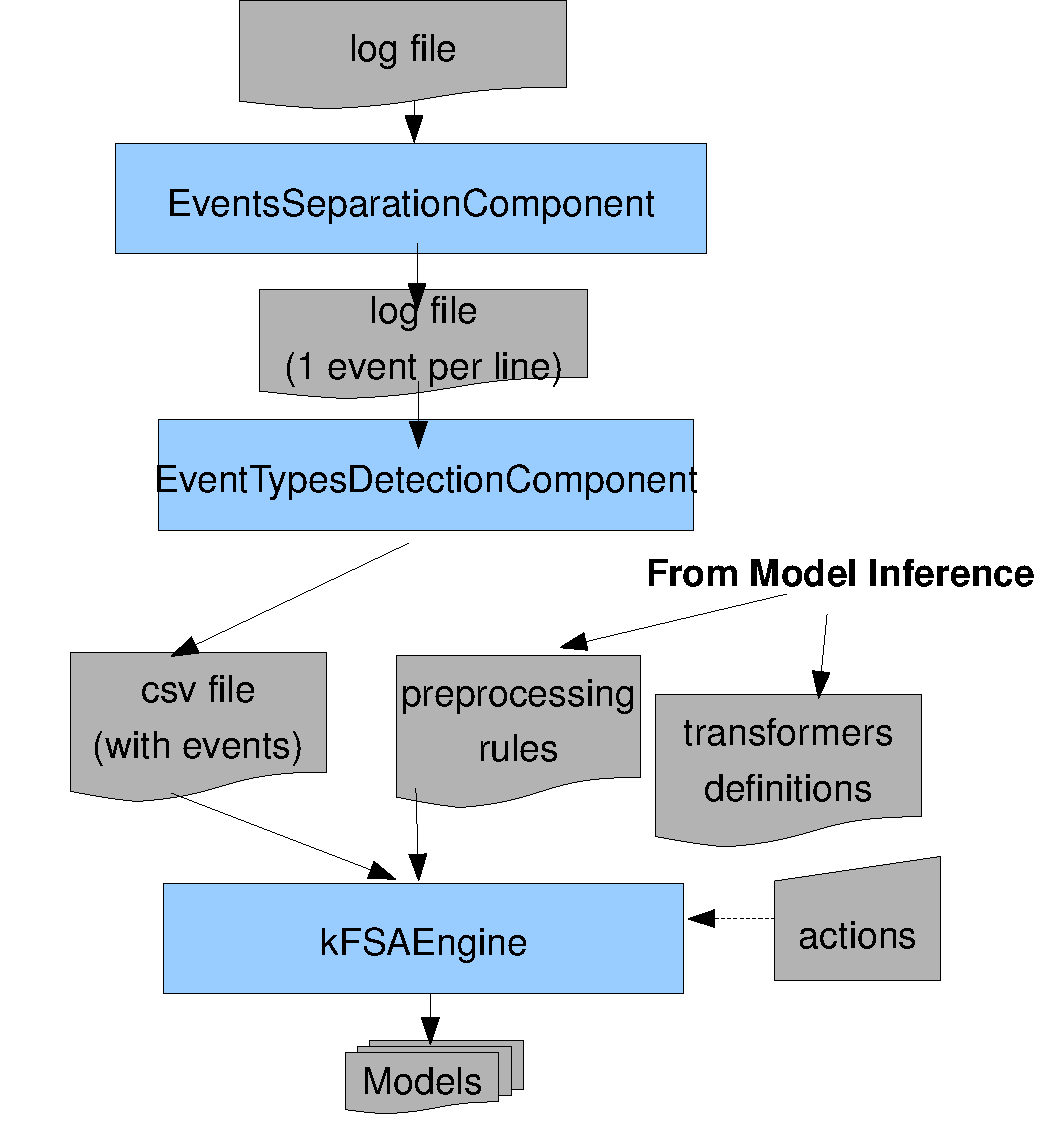
\includegraphics[width=13cm]{images/failureAnalysis}
    \end{center}
    \caption{Components involved in the failure analysis phase.}
\label{fig:failureAnalysis}
\end{figure*}

\subsubsection*{Raw Events Separation}

The command used to separate raw events is the same as in the ModelGeneration
phase except from the input and output parameters.


\begin{verbatim}
java -cp
path/to/klfa
preprocessing.rawEventsSeparation.RegexBasedRawEventsSeparator 
-eventStartExpression "\[#\|2008.*" ../faultyLogs/server.fail.log
events.fail.txt
\end{verbatim}

From \texttt{examples/glassfishForumUserIssue/analysis/} you can simply run
\texttt{../bin/run\-RawEventsSeparationChecking.sh}.

\subsubsection*{Events Types Detection}

The command is similar as in the Model Generation phase except from
the fact that we tell the tool to use the component and rules ids
used in the Model Generation phase. 

\textbf{Component Level Analysis}
\begin{verbatim}
 java -cp
path/to/klfa
it.unimib.disco.lta.alfa.preprocessing.eventTypesDetection.AutomatedEventTypesDetector
-replacement "CORE5076: Using.*" "Using Java" -replacement
".*/domains/domain1/config/" "/domains/domain1/config/" -replacement
"service:jmx:rmi:///jndi/rmi://.*:8686/jmxrmi" "" -replacement
"service:jmx:rmi:///jndi/rmi://.*:8686/jmxrmi" "" -replacement
"\|INFO\|" "" -replacement "\|FINE\|" "" -replacement "\|DEBUG\|" ""
-replacement "\|FINEST\|" "" -replacement "\|FINER\|" ""
-dataExpression "\[#\|2008.*\|.*\|.*\|.*\|.*\|(.*)\|#\]"
-componentExpression "\[#\|2008.*\|.*\|.*\|(.*)\|.*\|.*\|#\]" 
-loadComponents components.training.properties -exportRules
rules.checking.properties -workingDir checkingCsvGen
-loadEventPatterns -patternsDir trainingCsvGen
-componentsDefinitionFile components.fail.properties events.fail.txt
events.fail.csv

\end{verbatim}

From \texttt{examples/glassfishForumUserIssue/analysis/} you can simply run
../bin/runComponentLevelEventsDetectionChecking.sh.

\textbf{Application Level Analysis and Action Level Analysis}

\begin{verbatim}
 java -cp
path/to/klfa
it.unimib.disco.lta.alfa.preprocessing.eventTypesDetection.AutomatedEventTypesDetector
-dontSplitComponents -replacement "CORE5076: Using.*" "Using Java"
-replacement
".*/domains/domain1/config/" "/domains/domain1/config/" -replacement
"service:jmx:rmi:///jndi/rmi://.*:8686/jmxrmi" "" -replacement
"service:jmx:rmi:///jndi/rmi://.*:8686/jmxrmi" "" -replacement
"\|INFO\|" "" -replacement "\|FINE\|" "" -replacement "\|DEBUG\|" ""
-replacement "\|FINEST\|" "" -replacement "\|FINER\|" ""
-dataExpression "\[#\|2008.*\|.*\|.*\|.*\|.*\|(.*)\|#\]"
-componentExpression "\[#\|2008.*\|.*\|.*\|(.*)\|.*\|.*\|#\]" 
-loadComponents components.training.properties -exportRules
rules.checking.properties -workingDir checkingCsvGen
-loadEventPatterns -patternsDir trainingCsvGen
-componentsDefinitionFile components.fail.properties events.fail.txt
events.fail.csv

\end{verbatim}

From \texttt{examples/glassfishForumUserIssue/analysis/} you can simply run
../bin/runApplicationtLevelEventsDetectionChecking.sh or
../bin/runActionLevelEventsDetectionChecking.sh.

\subsubsection{Comparison against the models}

Comparison against the model is done calling the LogTraceAnalyzer
tool and giving the analysis type used in the model generation phase
and specifying that we are now doing the comparison.

\textbf{Component Level Analysis}

\begin{verbatim}
java -cp path/to/klfa tools.kLFAEngine.LogTraceAnalyzer
-separator "," -minimizationLimit 100 componentLevel checking
transformersConfig.txt preprocessingRules.txt events.fail.csv
\end{verbatim}

From \texttt{examples/glassfishForumUserIssue/analysis/} you can simply run
../bin/runComponentLevelAnomalyDetection.sh.

\textbf{Action Level Analysis}

\begin{verbatim}
 java -cp path/to/klfa
tools.kLFAEngine.LogTraceAnalyzer -separator "," -minimizationLimit
100 actionLevel checking transformersConfig.txt
preprocessingRules.txt events.correct.csv
\end{verbatim}

From \texttt{examples/glassfishForumUserIssue/analysis/} you can simply run
../bin/runActionLevelAnomalyDetection.sh.

\textbf{Application Level Analysis}

\begin{verbatim}
 java -cp path/to/klfa
tools.kLFAEngine.LogTraceAnalyzer -separator "," -minimizationLimit
100 applicationLevel checking transformersConfig.txt
preprocessingRules.txt events.correct.csv
\end{verbatim}

From \texttt{examples/glassfishForumUserIssue/analysis/} you can simply run
../bin/runApplicationLevelAnomalyDetection.sh.

\subsubsection{Anomalies interpretation}

In the model comparison phase the tool detects the anomalies present
in the faulty log files and report them to the user by saving them in
the file \texttt{klfaoutput/anomalies.csv}.

The last phase of the technique involves actively the user who has to
inspect the reported anomalies, and use them as a guide to inspect
correct and faulty files to detect the problem.

Table~\ref{analysisRes} shows the anomalies detected by the tool in
the
given case study.We imported the csv file produced by the tool,
anomalies.csv, and sorted the items according to the column
\texttt{Original
Event Line}. In the next paragraphs we are going to interpret them to
give an exhaustive explanation of the problem. 
\begin{sidewaystable}
\label{analysisRes}
\caption{Anomalies detected by KLFA for the Glassfish case study}
\begin{tabular*}{21cm}{|p{1.5cm}|p{2cm}|p{0.7cm}|p{0.7cm}|p{1.5cm}|p{
3cm } |p { 3cm } |p{2cm}|p{3cm}|}
\hline
Comp.&Anomaly&Line&State&State Type&Event&Original log
line&Original log event&Expected\\
\hline
5&FinalState&1&q2&Existing&5\_R0065&15&5,R0065&
5\_R0064 5\_R0066\_\_0\_\_0\\
\hline
0&FinalState&5&q8&Existing&0\_R0055)&20&0,R0055&
0\_R0052) 0\_R0057)\\
\hline
GLOBAL&Tail&13&q109&Existing&14\_R0020\_\_0)&21
14,R0020,java\-petstore\-2.0\-ea5&&3\_R0032) $\lambda$\\
\hline
14&FinalState&1&q4&Existing&14\_R0020\_\_0)&21
14,R0020,java\-petstore-2.0-ea5&&14\_R0023)\\
\hline
4&Tail&7&q12&Existing&4\_289331648)&24&4,289331648&
4\_-1628344215) 4\_R0073) 4\_1573705168 4\_R0075) \\
\hline
17&Tail&1&q3&Existing&17\_-811928006)&25&17,-811928006
&17\_R0003);\\
\hline
3&Tail&5&q10&Existing&3\_-1648356848)&27&3,-1648356848
&3\_R0032) 3\_R0031) \\
\hline
23&New Component&&&&&&&\\
\hline
\end{tabular*}

\end{sidewaystable}


\textbf{Anomaly 1}
Anomaly 1 appears in line 15 of the faulty log file. The anomaly
regards
 component \texttt{com.sun.jbi.framewor} 
(the id 5 correspond to
this component as you can see from file
\texttt{components.training.properties}). In this case the anomaly is
not caused by an unexpected event, but the system detects that the
events regarding component 5 stopped before expected. In fact a
new final state was added to the automaton.
By opening the automaton with the command \texttt{java -cp
path/to/klfa
tools.ShowFSA klfaoutput/5.fsa} we can see that many more events are
expected. Furthermore by looking at the faulty log file we can see
that the file is very short, so we can deduce that it was truncated
by the user or the application was blocked.

The \texttt{Event} column
in this case do not represent the wrong event occurred but the last
event seen. The id of this last event is R0065, which correspond to
the event regex
"JBIFW0010 JBI framework ready to accept requests.". 

\textbf{Anomaly 2} 
Anomaly 2 regards component \texttt{javax.enter\-prise.system.core},
also in this case the anomaly is caused by the premature end of
messages.

\textbf{Anomaly 3} 
Anomaly 3 regards component GLOBAL. This is not a real component, it
is a keyword used to indicate the automata that describes the way
components execution alternate.

The anomaly type is Tail, it indicates that an unseen tail was added
to the state q109. The first anomalous event seen is 14\_R0020\_0,
while it expected 3\_R0032, 3\_R0031, 13\_1394096499, or
2\_-2135717321
(the last three are detected following the $\epsilon$ transition).
The more interesting is the first one, which indicates that a deploy
message from component 3
(\texttt{javax.enterprise.system.to\-ols.admin}) is
missing from the log. We do not know if it indicates the cause of the
failure (This anomaly could depend on the fact that in one case it was used
the Glassfish \texttt{asadmin} tool while in the other not).

\textbf{Anomaly 4} 
Anomaly 4 regards component 14: the component recorded
less messages than expected. This is because the premature end of the
log file. KLFA expected a message of type R0023 (\texttt{\^(.*)
AutoDeploy Disabling AutoDeployment service.}), before
stopping the Glassfish server. We have an anomaly because in this log the
stopping phase of the server is not recorded.

\textbf{Anomaly 5} 
Anomaly 5 indicates that at line 24 an anomalous event 4\_289331648
occurs. The event ID in this case is an hash. The
AutomatedEventTypesExtractor assigns to a raw event line its hashcode
as its id when the raw event is an outlier. We have an outlier when a
raw event does not match any event regexp. 

The occurrence of an
hashcode as an anomalous event can have two meanings: the specific
event
was never seen in the correct logs analyzed or the event was
present in the logs analyzed but its was present very few time and it
was not considered an event type (by default this happens when an
event occurs just once). In the first case it can be an exceptional
event that appear as a consequence of a failure, or it can be a false
positive caused by event regexp that do not generalize enough the
data. This should happen if in the correct log files we have events in
which a parameter remains constant over all their occurrences: in
this case the parameter will be considered by SLCT as part of the
event regex, and in case the value change in the faulty execution
because of environmental reasons (e.g. domain of a web server) it
will be detected as an anomaly which may be not related to the
experienced failure (pay attention it should also be the case in
which in the correct execution the system was behaving correctly
because of this constant value).

In this case to further inspect the anomalous event we need to take a
look at the faulty log
file (\texttt{events.fail.txt}), we see that there is an
exception in line 24, which is related to the failure. The exception was
never seen in the correct log files (search for 289331648 in the
correct log).


\textbf{Anomaly 6} 
Anomaly 6 occur at line 25, the event 17\_-811928006 was unexpected.
As in the previous case the hashcode-id was generate because of a
message never seen before (the exception).

\textbf{Anomaly 7} 

Anomaly 7 is detected in line 27 of the trace file. Also in this case
if we take a look at the faulty log
file (\texttt{events.fail.txt}), in line 27 we see that there is an
exception, which is related with the failure. The technique has
detected an useful information for the root cause analysis.

\textbf{Anomaly 8} 

Anomaly 8 indicates that a new component appeared. If we open
\texttt{components.\-fail.\-properties} we see that component id 23
correspond to component
\texttt{com.sun.org.\-apache.commons.\-modeler.Registry}. By
looking for
it in the failure log we see that it appears because of an event
occurred as a consequence of the failure.



